%! Author = borisdeletic
%! Date = 03/05/2023

% Preamble
\documentclass[11pt]{article}

% Document
\begin{document}

\section{Parameter Adaption}\label{param_adaption}
    The sampling performance of Constrained HMC is heavily dependent on a number of parameters which must be finely
    tuned in order to extract the full potential of the algorithm.
    Namely, the step size $\epsilon$, path length $L$, and kinetic energy metric $M$ are very important and their
    optimal value depends on the distribution being sampled~\cite{MCMChamiltonian}.
    Manually choosing fixed values requires significant domain knowledge and is prone to human error.
    Schemes have been developed to adaptively set these parameters for HMC, such as the No-U-Turn
    criterion~\cite{hoffman2011nouturn} for choosing path lengths, and dual averaging~\cite{nesterov_dual_averaging}
    for setting the step size.

    Furthermore, in the case of CHMC for nested sampling it is not possible to use a fixed value for the
    step size $\epsilon$ and kinetic energy metric $M$, which maintains performance until termination.
    In nested sampling, after each iteration the iso-likelihood boundary is contracted, thereby implicitly changing the
    posterior distribution being sampled.
    Even if an optimal value for the step size is initially chosen, as the posterior space is compressed, the step size
    will unsuspectingly become too large and the integrator will lose efficiency until all new samples are rejected.

    \begin{figure}[t!]
        \center
        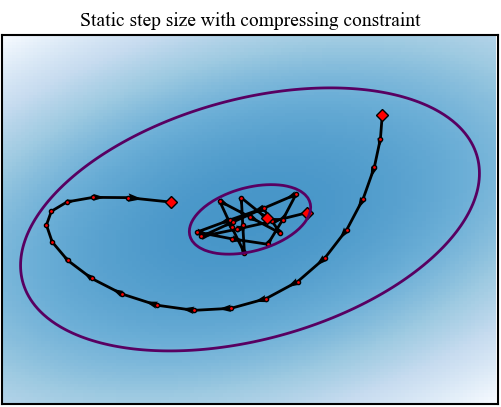
\includegraphics[width=\linewidth]{../figures/StaticStepSize}
        \caption{
            Trajectories for static step size $\epsilon$ with different iso-likelihood contours.
            $\epsilon$ may initially begin well tuned to explore the posterior, but as nested sampling iterates,
            the space compresses and sampling becomes inefficient.
            Eventually, CHMC will no longer be able to generate new samples with the given step size.
        }\label{fig:static_step_size}
    \end{figure}

    \subsection{Epsilon Dual Averaging}
    When choosing a value for $\epsilon$, a value that is too small will result in excessive computation time to explore
    the distribution, and a value that is too large will cause large rejection rates.
    We can use the Markov-Chain samples themselves to adapt $\epsilon$ to give a target Metropolis acceptance rate equal to $\delta$.
    Employing the dual averaging scheme of Nesterov~\cite{nesterov_dual_averaging} has been shown to be well suited
    to MCMC samplers due the convexity of giving proportionate weight to \emph{later} samples~\cite{hoffman2011nouturn}.

    Given statistics $H_t$, we want to find a parameter $x$ such that $\mathbb{E}_t[H_t|x] = 0$.
    We can apply the updates
    \begin{equation}\label{eq:dual_averaging}
    \begin{aligned}
        x_{t+1} &\gets \mu - \frac{1}{\gamma \sqrt{t}} \sum_{i=1}^t H_i \\
        \bar{x}_{t+1} &\gets \eta_t x_{t+1} + (1 - \eta_{t+1}) \bar{x}_t
    \end{aligned}
    \end{equation}

    where $\mu$ is a user defined parameter that $x_t$ is shrunk towards, $\gamma$ is a free parameter that controls
    the amount of shrinkage to $\mu$, and $\eta_t \equiv t^{-\kappa}$ is the shrinkage step size.

    To apply this averaging scheme to CHMC we set $x = \log{\epsilon}$ and $H_t = \delta - P_t$, where $P_t$ is the
    metropolis acceptance probability of sample $t$ and $\delta \in (0, 1)$.
    The values for $\mu, \kappa, \delta$ used for our implementations are listed in appendix~\ref{sec:paramvalues}.
    Averaging in HMC is generally performed for a fixed number of steps during the burn-in phase, after which the
    tuned value of epsilon is chosen and kept constant.
    As illustrated above, this scheme is modified for CHMC and we continuously adapt $\epsilon$ accordingly until termination.


    \subsection{Kinetic Energy Adaption}
    The kinetic energy term in the Hamiltonian\ref{} is expressed as
    \begin{equation}\label{eq:kinetic_energy}
    \begin{aligned}
        T = \frac{1}{2} \mathbf{p}^T M^{-1} \mathbf{p},
    \end{aligned}
    \end{equation}
    with metric $M$, where the momentum is drawn from the distribution $\mathbf{p} \sim \mathcal{N}(0, \sigma = M)$.
    Rephrasing the Hamiltonian in terms of energy $H(E)$, the metric defines which energy level sets will be explored
    by the HMC Markov-Chain.
    A poorly chosen metric will very slowly explore the energy levels of the target distribution $\pi(E)$.
    Schemes to diagnose suboptimal metrics for HMC have been developed using Bayesian information
    arguments~\cite{betancourt2016energymetric}, and geometric approaches~\cite{bales2019_hmc_metric}.

    We propose a new algorithm to continuously adapt the metric in CHMC for nested sampling, using motivations
    from \emph{equipartition theorem}.
    The equipartition theorem states that in thermal equilibrium, the energy is shared equally amongst a system's degrees
    of freedom~\cite{landau1972theoretical}.
    Considering the set of live points as a thermodynamic ensemble, we can therefore relate the \emph{variance} of the
    kinetic and potential energy distributions.
    \begin{equation}\label{eq:equipartition_theorem}
        \mathrm{Var}[T] = \mathrm{Var}[U].
    \end{equation}
    Following the derivation in~\ref{sec:metric_derivation} we arrive at the result for the metric
    \begin{equation}\label{eq:metric_adaption}
        M = \frac{2}{D} \sqrt{\mathrm{Var}[U]} \mathbb{1},
    \end{equation}
    Where $D$ is the dimensionality of the problem, and we use a scaled unit metric for simplicity.

    In order to computationally estimate the potential energy variance during the CHMC algorithm, we use the
    set of live points as an ensemble sample of the distribution.
    For example, when sampling directly from the posterior, $\mathrm{Var}[U] = \mathrm{Var}[\log{\mathcal{L}}]$,
    and we can update our metric every $\mathcal{O}(n_{live})$ iterations with very little computational overhead.

    We compared this scheme for kinetic energy adaption to other suggested approaches such as a BFMI
    diagnostic~\cite{betancourt2016energymetric}.
    We observe heuristically that our equipartition scheme performs better than BFMI, with lower
    computational cost, as we exploit the natural information contained by the set of live points.


\end{document}